\documentclass[UTF8,aspectratio=169,mathserif]{beamer}
\usepackage{ctex}
\usepackage{ulem}
\usepackage{color}
\usepackage{amssymb}
\usepackage{amsmath}
\usetheme{Berlin}
\setbeamertemplate{navigation symbols}{}

\title{7 - 随机计算}
\subtitle{Randomized computation}
\author{报告人:许博}
\date{2021年5月12日}

\begin{document}
	
	\begin{frame}
		\titlepage
	\end{frame}

	\begin{frame}{目录}
		\tableofcontents
	\end{frame}

	\section{概率图灵机和类$\bf BPP$}
	\begin{frame}{随机算法}{Randomized Algorithm}
		随机算法是可能涉及随机选择的算法。\newline
		
		实际中,随机算法使用随机数生成器实现,\newline 而事实上一个能够投掷公平硬币的生成器就足够了。
	\end{frame}
	
	\begin{frame}{概率图灵机}{Probabilistic Turing Machines}
		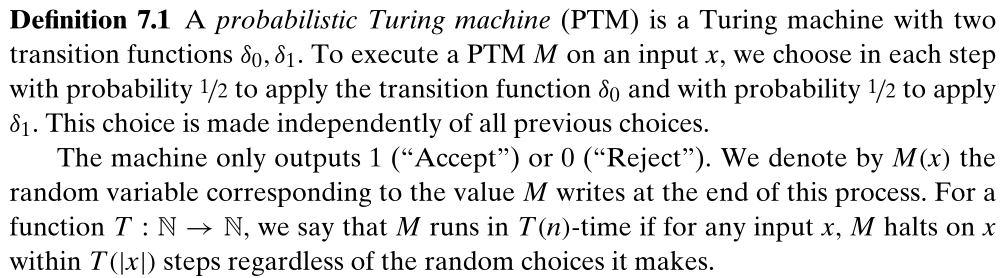
\includegraphics[width=\linewidth]{../../7/note.assets/image-20210508132612511.png}\newline
		
		PTM 和 NDTM 句法相似( syntactically similar),但概念上更像 DTM。
	\end{frame}
	
	\begin{frame}{类$\bf BPP$}{\textbf{B}ounded-error \textbf{P}robabilistic \textbf{P}olynomial-time}
		对 $L\subseteq\{0,1\}^*$ 和 $x\in\{0,1\}^*$,定义 $L(x)=1$ 如果 $x\in L$,否则 $L(x)=0$。\newline
		
		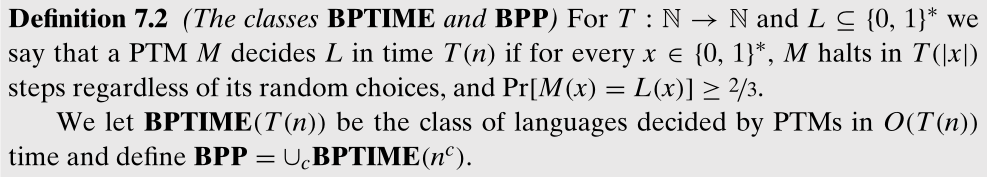
\includegraphics[width=\linewidth]{../../7/note.assets/image-20210508132647720.png}\newline
		
		$\bf BPP$ 类似 $\bf P$,仍然限制最坏情况下的复杂性。有$\bf P\subseteq BPP$。
	\end{frame}

	\begin{frame}{使用 DTM 定义 $\bf BPP$}
		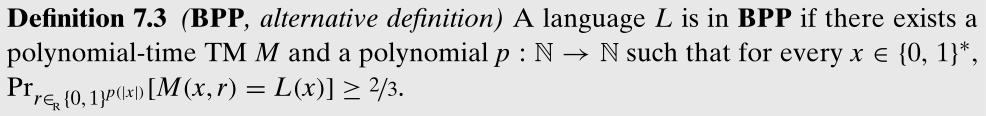
\includegraphics[width=\linewidth]{../../7/note.assets/image-20210508142316582.png}\newline
		
		有 $\bf BPP\subseteq EXP$。\newline
		
		${\bf BPP}=?\ {\bf P}$
	\end{frame}
	
	\section{一些 PTM 的例子}
	\begin{frame}{查找第 $k$ 小的数}{Finding the $k$-th Smallest Number}
		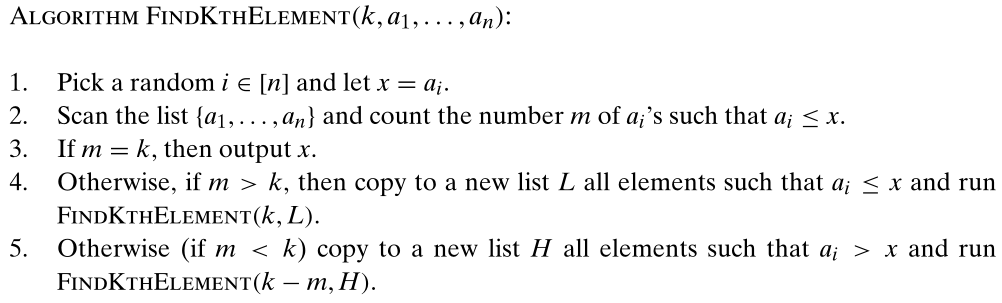
\includegraphics[width=\linewidth]{../../7/note.assets/image-20210508183753819.png}
	\end{frame}

	\begin{frame}{概率素数检测}{Probabilistic Primality Testing}
		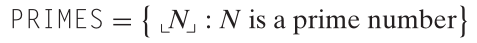
\includegraphics[width=0.4\linewidth]{../../7/note.assets/image-20210508190017980.png}\newline
		
		对整数 $N$,以及 $A\in[N-1]$,定义 $QR_N(A)$:
		
		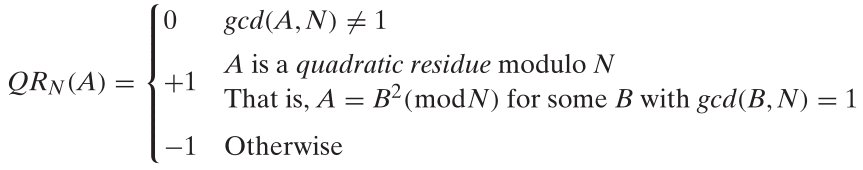
\includegraphics[width=0.7\linewidth]{../../7/note.assets/image-20210508203151275.png}\newline
		
		对奇数 $N$ 和 $A$,定义 $(\frac{N}{A}):=\Pi^k_{i=1}QR_{P_i}(A)$,其中 $P_i$ 是 $N$ 的所有质因子。
	\end{frame}

	\begin{frame}{概率素数检测}{Probabilistic Primality Testing}
		算法:对于一个随机的 $1\le A<N$,如果 $gcd(N,A)>1$ 或 $(\frac{N}{A})\neq A^{(N-1)/2}$,则判断 $N$ 为合数;否则认为 $N$ 是素数。\newline
		
		$N$ 是素数时一定满足 $gcd(N,A)=1$ 和 $(\frac{N}{A})=A^{(N-1)/2}$;$N$ 是奇合数时,满足 $gcd(N,A)=1$ 的 $A$ 中仅有最多一半能够令 $(\frac{N}{A})=A^{(N-1)/2}$,因此合数同时满足这两个条件的概率小于 $1/2$。
	\end{frame}
	
	\begin{frame}{多项式恒等检测,Polynomial Identity Testing}
		\begin{block}{代数电路}
			类似布尔电路,但运算为 $+,-,*$。代数电路定义了一个由 $\mathbb{Z}^n$ 到 $\mathbb{Z}$ 的多项式。
		\end{block}
		
		\begin{block}{ZEROP}
			定义 ZEROP 为计算恒等于零的多项式的代数电路的集合。
		\end{block}
	
		\begin{block}{Schwartz-Zippel Lemma}
			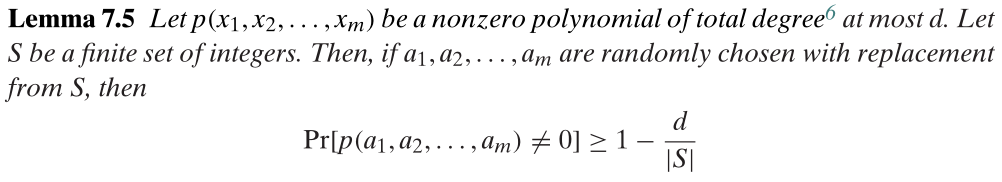
\includegraphics[width=\linewidth]{../../7/note.assets/image-20210509094630024.png}
		\end{block}
	\end{frame}

	\begin{frame}{多项式恒等检测}{Polynomial Identity Testing}
		一个大小为 $m$ 的电路 $C$ 可以包含最多 $m$ 个乘法,即定义一个次数最多为 $2^m$ 的多项式。\newline
		
		一个简单的概率算法:从 1 到 $10*2^m$ 中选择 $n$ 个数 $x_1,...,x_n$,求电路 $C$ 在 $x_1,...,x_n$ 上的值 $y$,如果 $y=0$ 则接受,否则拒绝。\newline
		
		显然如果 $C\in{\rm ZEROP}$,则总是接受。而如果 $C\notin{\rm ZEROP}$,至少有 $9/10$ 的概率会拒绝。因为 $d<2^m$,而 $|S|=10*2^m$,因此 $Pr(p\neq0)\ge\cfrac{9}{10}$。
	\end{frame}

	\begin{frame}{多项式恒等检测}{Polynomial Identity Testing}
		问题:输出的大小可能为 $(10*2^m)^{2^m}$,即 $2^m$ 个 $10*2^m$ 相乘。\newline
		
		解决方案:指纹(fingerprinting)技术。即在求值时模 $k$,$k$ 在 $[2^{2m}]$ 中随机选择,最后计算的值为 $y\ (mod\ k)$,显然如果 $y=0$,则 $y\ (mod\ k)$=0,而如果 $y\neq0$,则 $k$ 至少有 $\delta=\frac{1}{4m}$ 的概率不整除 $y$。可以通过重复这个过程 $O(1/\delta)$ 次,并且只有所有的输出都为 0 才接受来减小误差。
	\end{frame}

	\begin{frame}{二分图完备匹配检测}{Testing for Perfect Matching in a Bipartite Graph}
		令 $G=(V,E)$ 是一个二分图,其中 $V$ 可以分成两个大小相同的不相交子集 $V_1,V_2$,即 $V=V_1\cup V_2$,并有 $E\subseteq V_1\times V_2$,即 $G$ 中的每一个边的两个顶点都分别属于 $V_1$ 和 $V_2$。\newline
		
		$G$ 中的一个完备匹配是边的一个子集 $E'\subseteq E$ ,使得每个顶点在 $E'$ 中恰好出现一次。
	\end{frame}

	\begin{frame}{二分图完备匹配检测}{Testing for Perfect Matching in a Bipartite Graph}
		记 $n=|V_1|=|V_2|$,用集合 $[n]$ 标识这两个集合,可以把 $E'$ 看作是一个排列 $\sigma:[n]\rightarrow[n]$,映射每个 $i\in[n]$ 到一个唯一的 $j\in[n]$,使得 $\overline{ij}\in E'$。令 $X$ 是一个 $n\times n$ 的实变量矩阵,如果边 $\overline{ij}\in E$,则 $X_{i,j}$ 等于变量 $x_{i,j}$,否则 $X_{i,j}$ 等于 0。\newline
		
		一个矩阵 $A$ 的行列式定义为:
		
		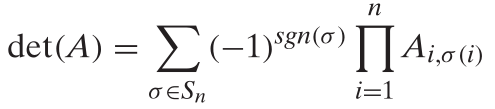
\includegraphics[width=0.4\linewidth]{../../7/note.assets/image-20210509123241893.png}\newline
		
		如果 $G$ 有完备匹配当且仅当 $det(X)$ 不是恒等于零的多项式。
	\end{frame}

	\begin{frame}{二分图完备匹配检测}{Testing for Perfect Matching in a Bipartite Graph}
		算法:从 $[2n]$ 中为 $x_{i,j}$ 选择值,在 $X$ 中替换并计算行列式,如果行列式非零,则判定输入的图有完备匹配,否则判定无。\newline
		
		对于一个无完备匹配的图,结果一定为零;而对于一个存在完美匹配的图,结果不为零的概率大于等于 $1-\frac{n}{2n}=\frac{1}{2}$,因为多项式中次数最多为 $n$。
	\end{frame}
	
	\section{单边误差和“零边”误差}
	\begin{frame}{双边误差}{Two-sided Error}
		双边误差的概率算法即允许用于语言 $L$ 的算法在 $x\in L$ 时输出 0 以及在 $x\notin L$ 时输出 1。\newline
		
		类 $\bf BPP$ 捕获了具有双边误差的概率算法。${\rm Pr}[M(x)=L(x)]\ge 2/3$
	\end{frame}

	\begin{frame}{单边误差,One-sided Error}
		单边误差的概率算法,即当 $x\notin L$ 时,算法不会输出 1,但仍可能在 $x\in L$ 时输出 0。\newline
		
		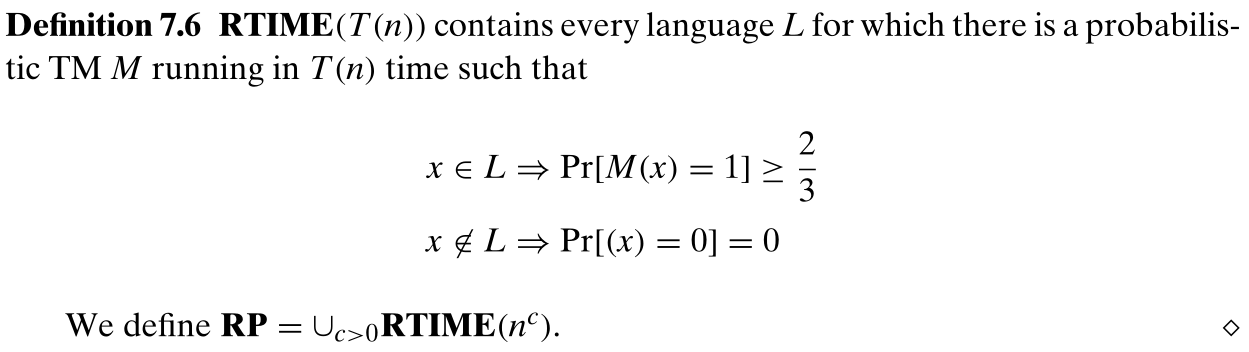
\includegraphics[width=\linewidth]{../../7/note.assets/image-20210509133757822.png}\newline
		
		有 $\bf RP\subseteq NP$。类 ${\bf coRP}=\{L|\overline{L}\in{\bf RP}\}$ 捕获“另一方向”的单边误差算法。
	\end{frame}

	\begin{frame}{零边误差}{Zero-sided Error}
		期望运行时间:对一个 PTM $M$ 及输入 $x$,随机变量 $T_{M,x}$ 为 $M$ 在 $x$ 上的运行时间,${\rm Pr}[T_{M,x}=T]=p$ 表示 $M$ 在 $x$ 上 $T$ 步内停机的概率是 $p$。如果对每个 $x\in\{0,1\}^*$ 期望 ${\rm E}[T_{M,x}]$ 最多为 $T(|x|)$,则称 $M$ 具有期望运行时间 $T(n)$。\newline
		
		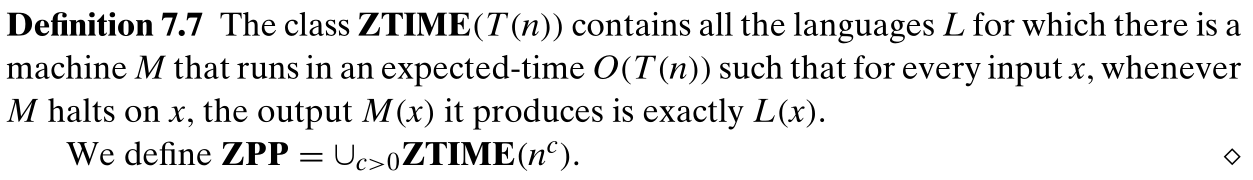
\includegraphics[width=\linewidth]{../../7/note.assets/image-20210509153030302.png}\newline
		
		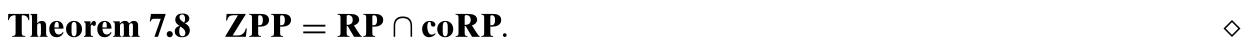
\includegraphics[width=\linewidth]{../../7/note.assets/image-20210509153059395.png}
	\end{frame}
	
	\section{定义的稳健性}
	\begin{frame}{精确常数的作用:减少误差}
		常数 $2/3$ 可以由任何大于 $1/2$ 的常数代替:\newline
		
		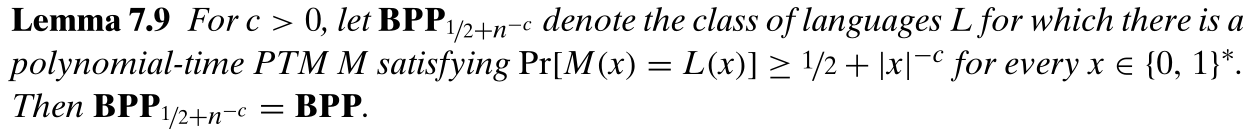
\includegraphics[width=\linewidth]{../../7/note.assets/image-20210509153425924.png}\newline
		
		通过若干次重复的主要结果作为输出,可以减小误差,提高结果的准确率。
	\end{frame}

	\begin{frame}{期望运行时间和最坏情况运行时间}
		定义 RTIME 和 BPTIME 时,要求机器在 T(n) 时间内停机,而不管它的随机选择,但是可以使用期望运行时间代替。\newline
		
		因为一个期望运行时间为 T(n) 的 PTM 可以变换为一个运行最多 100T(n) 步的 PTM,同时简单地增加一个计数器,在太多步之后以任意输出停止即可。而根据马尔可夫不等式,M 运行超过 100T(n) 步的概率最多为 1/100,因此这将使接受概率最多改变 1/100。
	\end{frame}

	\begin{frame}{允许更一般的随机选择}
		对于出现“heads”概率是 $\rho\neq\cfrac{1}{2}$ 的硬币,称之为 $\rho$-币。当 $\rho$ 是可高效计算(每一位可以多项式时间计算)的数时,掷$\rho$-币的概率算法的能力不会增加。\newline
		
		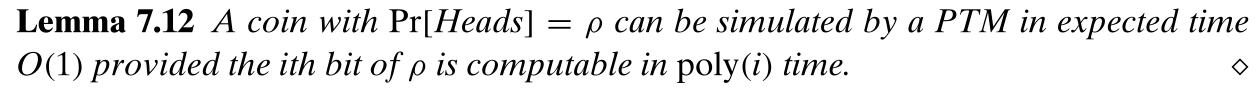
\includegraphics[width=\linewidth]{../../7/note.assets/image-20210509154955249.png}\newline
		
		相反的,掷$\rho$-币的概率算法的计算能力也不弱于标准概率算法。
	\end{frame}
	
	\section{随机规约}
	\begin{frame}{随机规约}
		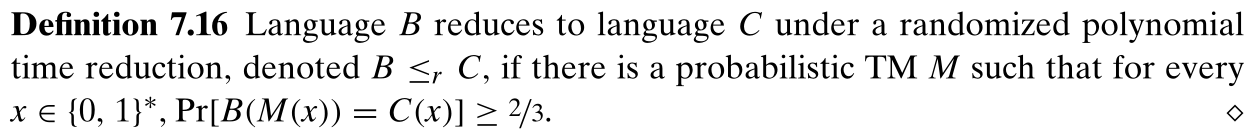
\includegraphics[width=\linewidth]{../../7/note.assets/image-20210509155949766.png}\newline
		
		$\bf NP$ 可以定义为集合 $\{L:L\le_p{\rm 3SAT}\}$,替换为 $\le_r$ 可以得到 $\bf BP$ 版本的 $\bf NP$ 定义:
		
		
\includegraphics[width=\linewidth]{../../7/note.assets/image-20210509162341964.png}
	\end{frame}

	\section{空间有界随机计算}
	\begin{frame}{类$\bf BPL$ 和 $\bf RL$}
		如果在任何计算分支中,使用的非空纸带最多为 $O(S(n))$,称一个 PTM 使用 $S(n)$ 的空间。类 $\bf BPL$ 和 $\bf RL$ 是类 $\bf L$ 的双边误差和单边误差的概率类似版本:\newline
		
		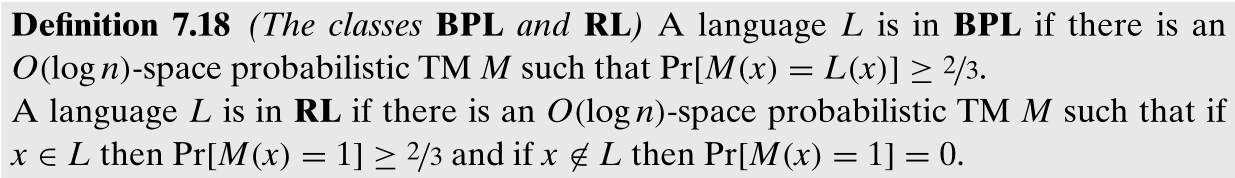
\includegraphics[width=\linewidth]{../../7/note.assets/image-20210509162758560.png}
	\end{frame}

	\begin{frame}{UPATH问题的$\bf RL$-算法}
		
\includegraphics[width=\linewidth]{../../7/note.assets/image-20210509163216637.png}
		
		\begin{block}{UPATH}
			给定一个 $n$ 个顶点的无向图,以及两个顶点 $s$ 和 $t$,判定 $s$ 和 $t$ 是否相连。
		\end{block}
		
		算法:从 $s$ 开始随机走长度为 $l=100n^4$ 的路径。也即初始化变量 $v$ 为 $s$,每一步随机选择 $v$ 的一个邻居 $u$,然后将 $u$ 赋值给 $v$。当且仅当在 $l$ 步内到达 $t$ 时接受。\newline
		
		对数空间,只需要存储顶点的编号。若 $s$ 与 $t$ 不相连,算法不接受;若 $s$ 和 $t$ 相连,则从 $s$ 走到 $t$ 的期望步数最多为 $10n^4$,接受的概率最少为 $3/4$。
	\end{frame}
		
\end{document}